\documentclass{amsart}
%\renewcommand{\baselinestretch}{2}

\usepackage{amssymb}
\usepackage{amsmath}
\usepackage{amsthm}
\usepackage{amsbsy}
\usepackage[dvips]{graphicx}
\usepackage{amscd}
\usepackage{bm}
\usepackage{mdframed}
\usepackage{siunitx}
\usepackage{hyperref}
\usepackage{url}
\usepackage{listings}

\theoremstyle{plain}
\newtheorem{theorem}{Theorem}[section]
\newtheorem{lemma}[theorem]{Lemma}
\newtheorem{corollary}[theorem]{Corollary}
\newtheorem{proposition}[theorem]{Proposition}
\newtheorem*{conjecture}{Conjecture}
\newtheorem*{exercise}{Exercise}

\theoremstyle{definition}
\newtheorem{definition}{Definition}[section]

\theoremstyle{remark}
\newtheorem{remark}[theorem]{Remark}
\newtheorem*{aside}{Aside}
\newtheorem*{acknowledgements}{Acknowledgements}
\newtheorem{example}{Example}[section]

\newcommand{\onto}{\twoheadrightarrow}
\newcommand{\del}{\partial}
\newcommand{\incl}{\hookrightarrow}
\newcommand{\Incl}{\hookleftarrow}
\newcommand{\F}{\mathfrak{F}}
\newcommand{\FF}{\mathcal{F}}
\newcommand{\G}{\left\vertG\right\vert}
\newcommand{\Z}{{\mathbb{Z}}}
\newcommand{\C}{{\mathbb{C}}}
\newcommand{\N}{{\mathbb{N}}}
\newcommand{\R}{{\mathbb{R}}}
\renewcommand{\P}{{\mathfrak{P}}}
\renewcommand{\H}{{\mathbb{H}}}
\newcommand{\Zp}{\mathbb{Z}/p\mathbb{Z}}
\newcommand{\Zq}{\mathbb{Z}/q\mathbb{Z}}
\newcommand{\Zz}{\mathbb{Z}/2\mathbb{Z}}
\newcommand{\sm}{\setminus}
\renewcommand{\i}{\bm{i}}
\renewcommand{\j}{\bm{j}}
\renewcommand{\k}{\bm{k}}
\newcommand{\TG}{\Theta_3(\del G)}
\newcommand{\TM}{\Theta_3(M)}
\newcommand{\co}{\colon\thinspace}
\newcommand{\impl}{\Rightarrow}

\begin{document}

\title[Euclidean Geometry by High-performance Solvers?]{Euclidean Geometry by\\ High-performance Solvers?}
\date{\today}
\author{Siddhartha Gadgil}

\address{Department of Mathematics\\
	Indian Institute of Science\\
	Bangalore.}
\email{gadgil@iisc.ac.in}

\author{Anand Tadipatri}
\address{Indian Institute of Science Education and Research\\
	Pune.}

\begin{abstract}
	Tarski showed in the 1950s that (first-order) questions in Euclidean geometry can be answered algorithmically. 
	Algorithms for doing this have greatly improved over the decades, but still have high complexity (in terms of time taken). 
	We experiment with using state-of-the art software, specifically so called \emph{SMT Solvers}, to see how practical it is 
	to prove classical Euclidean geometry results in this way. 
\end{abstract}

\maketitle

Computers are able to solve an increasing range of problems, many of
which were believed not long ago to require human intelligence and creativity. Yet
there are fundamental limitations to what problems can be solved
algorithmically. In particular, by
results of G\"odel, Turing, Church and others, there is no computer
program that, given a mathematical statement as input, either gives a
proof or (correctly) says that the statement is false.

Indeed, we cannot algorithmically solve even a seemingly simple class of
problems: deciding whether (systems of) so called
\emph{Diophantine Equations} have solutions. A Diophantine equation is a polynomial
equation with integer coefficients, such as $n^2 + m^2 = 3$ or \(3n^2 + 7m^2 = r^3\).
Solutions of such equations are assignments of \textbf{integers} to the variables so that
the equations (or systems of equations) are satisfied.
We say that a Diophantine equation (or a system of Diophantine equations) is \emph{satisfiable}
if it has (integral) solutions.
For
instance, we can see that the Diophantine equation \(n^2 + m^2 = 3\) is not satisfiable,
since there are no integers $n$ and $m$ with \(n^2 + m^2 = 3\), even though there
are many pairs of real numbers that satisfy this -- these indeed form a circle (renaming the variables
to $x$ and $y$ gives the familiar equation $x^2+ y^2 =3$ of a circle with radius $\sqrt{3}$).

As a result of combined work of Martin Davis, Yuri Matiyasevich, Hilary
Putnam and Julia Robinson during the 1950s and 1960s, we know that there
is no algorithm (i.e., computer program) to which we can input the
coefficients of a Diophantine equation and which will tell us
(correctly) whether the equation has integral solutions.

Yet, the above results should not be over-interpreted to say that proofs
cannot be found by programs. Indeed if we turn from numbers to the other
classical source of mathematics -- Euclidean geometry, the situation is
different. Using coordinate geometry, geometric figures can be described by equations,
and geometric problems can be translated (as we illustrate in this article) into
\emph{satisfiability} problems for systems of \textbf{real} equations and inequations. Thus, we
associate to a geometric problem equations and inequations with real coefficients,
with satisfiability meaning that we can
assign real values to the variables so the equations and inequations are satisfied.
A geometric statement is universally false (i.e., the statement never holds) if and only if the corresponding equations and inequations are \emph{unsatisfiable}. Thus, to prove a theorem in geometry, one can translate the negation of the theorem statement into a system of equations and inequations and verify that it is unsatisfiable (i.e., there are no real solutions).

In the 1950s, Tarski proved that whether a (finite)
collection of polynomial equations and inequations has solutions that
are real numbers is algorithmically decidable.  Tarski's algorithm has been greatly improved,
and algorithms of a more algebraic nature have also been developed,
improved and implemented. Yet they remain slow.

This article is about our experiments to use
state-of-the-art solvers to try in practice to prove such results.
These experiments were prompted by a lecture
to undergraduate students, during which \href{https://github.com/Z3Prover/z3}{\texttt{Z3}}, a high-performance
solver from Microsoft (which is open source), was used to solve a Sudoku problem (a standard demo for this technology). The puzzle was duly solved instantly. You can see such
a demo \href{https://rise4fun.com/Z3/Cs7p}{online}, but the online
version is slow.

Since we could not find examples of geometric theorems proved using \texttt{Z3} or
its friends, we decided to try proving
some results in this way. Specifically we attempted the \emph{Pappus hexagon theorem}
(which has deep connections to modern mathematics) and \emph{Menelaus's theorem}.

Our results were mixed -- with \texttt{Z3} able to answer the satisfiability problem,
but not when it was asked to give a solution with proof.
Especially as these systems are vastly improving, it seems worthwhile to
write about how such systems can be used at least in principle,
especially since this does not seem to be widely known. We remark that the 
specific problems considered by us can also be investigated using symbolic algebra software such 
as Mathematica and Maple.

An interactive notebook with code for our examples is available online on Binder at 
\url{https://bit.ly/3e5bhfA}\footnote{Full link:\\\url{https://hub.gke2.mybinder.org/user/siddhartha-gadg-ing-mathematics-2x6efnix/notebooks/jupyter_notebook/SMTSolverDemonstration.ipynb}}.

\hypertarget{p-versus-np-and-satsmt-solvers}{%
	\section{P versus NP and \texttt{SAT}/\texttt{SMT}
	  solvers}\label{p-versus-np-and-satsmt-solvers}}

Some problems, such as solving a system of linear equations, are not
difficult, at least once one knows a method to solve them. The thumb
rule used is that if we can solve a problem with the number of steps
being at most a polynomial in the size of the problem (for instance, the
total number of digits in the coefficients of equations), then we
consider the problem to be easy enough. The class of these problems is
called \texttt{P} (i.e., Polynomial time).

A more interesting class of problems is ones for which we can
\emph{check} that a solution is correct reasonably easily, though it may
not be clear how to \emph{find} a solution in an easy manner. This is
typically the case with puzzles like jigsaws or Sudoku -- indeed the
appeal of puzzles perhaps lies in this feature. Such problems are called
\texttt{NP} problems (or problems in the class \texttt{NP}). While it appears that
many such problems do not have easy (i.e., polynomial time) solutions,
there is no proof of this. Whether every problem whose solution is easy
to check has a solution that is easy to find is the \texttt{P} versus \texttt{NP}
problem.

What makes the \texttt{P} versus \texttt{NP} problem specially interesting and fruitful is the
Cook-Levine theorem from the early 1970s. This says that if one specific
problem (which is in NP), called the \emph{Boolean satisfiability problem} (or
\(\texttt{SAT}\)), has a polynomial time solution, then \emph{every} problem that
is in \texttt{NP} can be solved in polynomial time. It can be deduced that
there are many other problems with the same property. Such problems are
called \texttt{NP}-complete.

\subsection{Boolean satisfiability (\texttt{SAT})}

The Boolean satisfiability problem (\(\texttt{SAT}\)) is similar to the satisfiability
problems for Diophantine or real equations, with \emph{Boolean} variables.
This means that the variables take values \emph{true} and \emph{false} -- we
can think of variables $P$, $Q$, ... representing whether some statements are
true or false. These can be combined using the logical operations \emph{and}
(denoted $P\wedge Q$), \emph{or} (denoted $P\vee Q$) and \emph{not} (denoted $\neg P$).
Combinations of the variables built using these give a collection of clauses, for example we
may have two variables $P$ and $Q$ and consider the clauses $P\wedge(\neg Q)$ and $(\neg Q)\vee P$.
The (finite) collection of clauses is satisfiable if we can assign true/false values to the variables
so that all the clauses are true. For example, the set of clauses $\{P\wedge(\neg Q), (\neg Q)\vee P\}$
is not satisfiable (which one can check by trying all $4$ possibilities for $P$ and $Q$).
Deciding whether a finite collection of clauses is satisfiable is
the \texttt{SAT} problem.


\subsection{\texttt{SAT} solvers}\label{sat-solvers}

While the theoretical \texttt{P} vs \texttt{NP} problem remains mysterious, the
Cook-Levine theorem has had some remarkable practical uses. Since so
many classes of problems can be reduced to solving one class of
problems, namely \(\texttt{SAT}\), a powerful approach has been to develop
various clever ways, and powerful programs incorporating them, to solve
\(\texttt{SAT}\) problems better, and then using these to solve other problems.
Such programs are called \emph{\(\texttt{SAT}\) solvers} .


While it appears that no program can solve all \(\texttt{SAT}\) problems
reasonably fast (i.e., in polynomial time), high-performance \(\texttt{SAT}\)
solvers try to solve as large a class of \(\texttt{SAT}\) problems as quickly as
possible in practice. Indeed in many cases a \(\texttt{SAT}\) problem may not be too
hard -- for example the problem becomes reasonably easy if there are either so
many solutions that one can readily find one or so many constraints that
one can readily show that there are no solutions.

\subsection{\texttt{SMT} Solvers}
\(\texttt{SMT}\) solvers (for \emph{Satisfiability Modulo Theories}) extend these
ideas to handle problems that involve not just Booleans, but also
integers and real numbers (and, in general, any first-order theories). Thus, we can require that a collection of
equations are satisfied, or a mixture of equations and inequations
(examples of inequations are \(x^2 < 3\), \(x^3 \geq 3z\), and
\(y^2 + z^2 \neq 1\)) or even a logical combination of these (for example,
(\(x^2 < 3)\vee(y^2 + z^2 \neq 1)\)). Again, many instances of these problems are hard, and there
are even ones with no algorithmic solution. Nevertheless the approach
taken is to solve as large a class of problems as efficiently as
possible.


\section{Geometry theorems as satisfiability problems}

We next describe how we translated statements of theorems from
Euclidean geometry into satisfiability results, suitable for using \texttt{SMT} solvers.

\subsection{The Pappus Hexagon theorem}
A theorem we attempted to prove was the \emph{Pappus hexagon theorem}, which
we now describe. In addition to being a typical geometry result, this
has a deeper mathematical meaning (corresponding to commutativity for
affine geometries over division rings), as you can read in the beautiful book~\cite{Ar}.

Suppose we are given two lines, with points \(a\), \(b\) and \(c\) on
the first line and \(A\), \(B\) and \(C\) on the second line as in
Figure~\ref{F:pappus}. We consider the general case, where no pair of lines
involving these points are parallel. Let \(P\) be the intersection of
the lines \(Ab\) and \(aB\), \(Q\) the intersection of \(Ac\) and
\(aC\), and \(R\) the intersection of \(Bc\) and \(bC\). The Pappus
hexagon theorem is the result that \(P\), \(Q\) and \(R\) are
\emph{collinear}, i.e., there is a line containing all three of these
points, for all choices of \(a\), \(b\), \(c\), \(A\), \(B\), and \(C\)
of the above form.

\begin{figure}
	\centering
	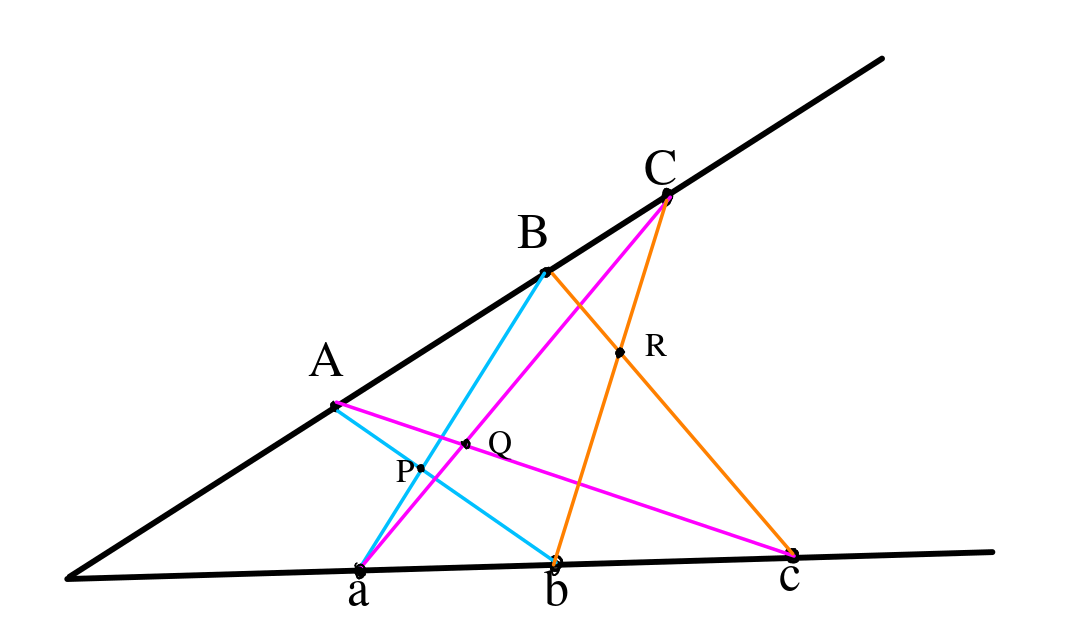
\includegraphics[scale=0.3]{Pappus.png}
	\caption{Pappus Theorem}\label{F:pappus}
\end{figure}

\hypertarget{equations-for-collinearity}{%
	\subsection{Equations for
		collinearity}\label{equations-for-collinearity}}

We shall formulate the Pappus theorem in terms of collinearity, and
then translate this into equations and inequations.
Recall that collinearity can be
expressed as a polynomial equality. Namely, points with coordinates
\((x_1, y_1)\), \((x_2, y_2)\) and \((x_3, y_3)\), which we assume to be
distinct, are collinear if and only if
\[\frac{y_2 - y_1}{x_2 - x_1} = \frac{y_3 - y_1}{x_3 - x_1}\] which is
equivalent to \[(y_2 - y_1)(x_3 - x_1) = (y_3 - y_1)(x_2 - x_1).\]

\subsection{Warmup: a simple problem}\label{a-simple-problem}

As a warmup and sanity check, we set up the problem of showing that for
an arbitrary point \(P = (x, y)\), the three points \(P=(x, y)\),
\(O=(0, 0)\) and \(-P=(-x, -y)\) are collinear.

We prove such results using \texttt{SMT} solvers by contradiction. In this case,
for variables \(x\) and \(y\), we impose the condition that the points
\(P\), \(O\) and \(-P\) are \emph{not} collinear. If the solver shows
that this cannot be satisfied, then it follows that the points are
always collinear. Observe that the condition of not being collinear just
means that equation in the above equation is replaced by the inequation
\((y_2 - y_1)(x_3 - x_1) \neq (y_3 - y_1)(x_2 - x_1)\).

Indeed the solvers \texttt{Z3} and \texttt{CVC4} (another \texttt{SMT} solver, and the champion in the
latest competition for \texttt{SMT} solvers) proved this result instantly -- more
precisely, \texttt{Z3} took \(0.012\) seconds and \texttt{CVC4} took \(0.094\) seconds.

\subsection{Formulating Pappus theorem using polynomial (in)equations}

We next translate the Pappus theorem, first into coordinate geometry and then into
real equations and inequations.

\subsubsection{Choosing coordinates}

While one can (and we initially did) take arbitrary coordinates for the
\(6\) points \(a\), \(b\), \(c\), \(A\), \(B\) and \(C\) and add
equations for their being collinear, we consider a simpler variant where
we choose coordinates and parametrize the points. Namely, we can take
\(a\), \(b\) and \(c\) on the \(x\)-axis with \(a = (1, 0)\). Then we have
\(b = (1 + u, 0)\) and \(c = (1 + u + v, 0)\) with \(u>0\) and \(v>0\).
Similarly, if we let \(A = (x_A, y_A)\), then we can assume that
\(B = (x_A(1+ U), y_A(1 + U))\) for some \(U > 0\) and
\(C = (x_A(1+ U + V), y_A(1 + U + V))\) for some \(V > 0\). Further, we
can assume that \(y_A > 0\).

Let the points \(P= (x_P, y_P)\), \(Q = (x_Q, y_Q)\) and
\(R= (x_R, y_R)\) have arbitrary coordinates. We add equations
corresponding to their being intersection points, as we see below. Thus,
we have \(12\) variables in all, \(6\) of them the parameters \(u\),
\(v\), \(x_A\), \(y_A\), \(U\) and \(V\) for the problem and \(6\) more
coordinates of the intersection points. Further, we have inequations
\(u >0\), \(v >0\), \(y_A >0\), \(U > 0\) and \(V >0\). We shall add to
these equations and inequations from the statement of the theorem.

\subsubsection{Equations and inequations}

We reformulate the Pappus hexagon theorem in terms of collinearity.
Observe that \(P\) being the intersection point of \(Ab\) and \(aC\) is
equivalent to both the triples of points \((A, P, b)\) and \((a, P, B)\)
being collinear. We have similar conditions for \(Q\) and \(R\). Thus,
the conditions on \(P\), \(Q\) and \(R\) can be formulated in terms of
collinearity of \(6\) triples of points.

Finally, the conclusion is that \(P\), \(Q\) and \(R\) are collinear. We
seek to prove this by contradiction, namely we add the condition that
they are not collinear, and show that the resulting system cannot be
satisfied. Again, the condition that the points are not collinear gives
an inequation.

In summary, we have a problem asking whether a set of algebraic
equations and inequations has a solution over reals. This system has
\(12\) variables, with \(6\) equations corresponding to collinearity,
\(5\) inequations stating that variables are positive and an inequation
(to contradict) stating that three points are not collinear.

We shall discuss the results of our attempts to prove this in Section~\ref{running-smt-solvers}.
Before that, we state, and translate into \texttt{SMT} form another geometric result, which 
we also tried to prove.

\subsection{Menelaus's theorem}

Another classical result in geometry is \emph{Menelaus's theorem}, formulated by Menelaus of Alexandria.

\begin{figure}
	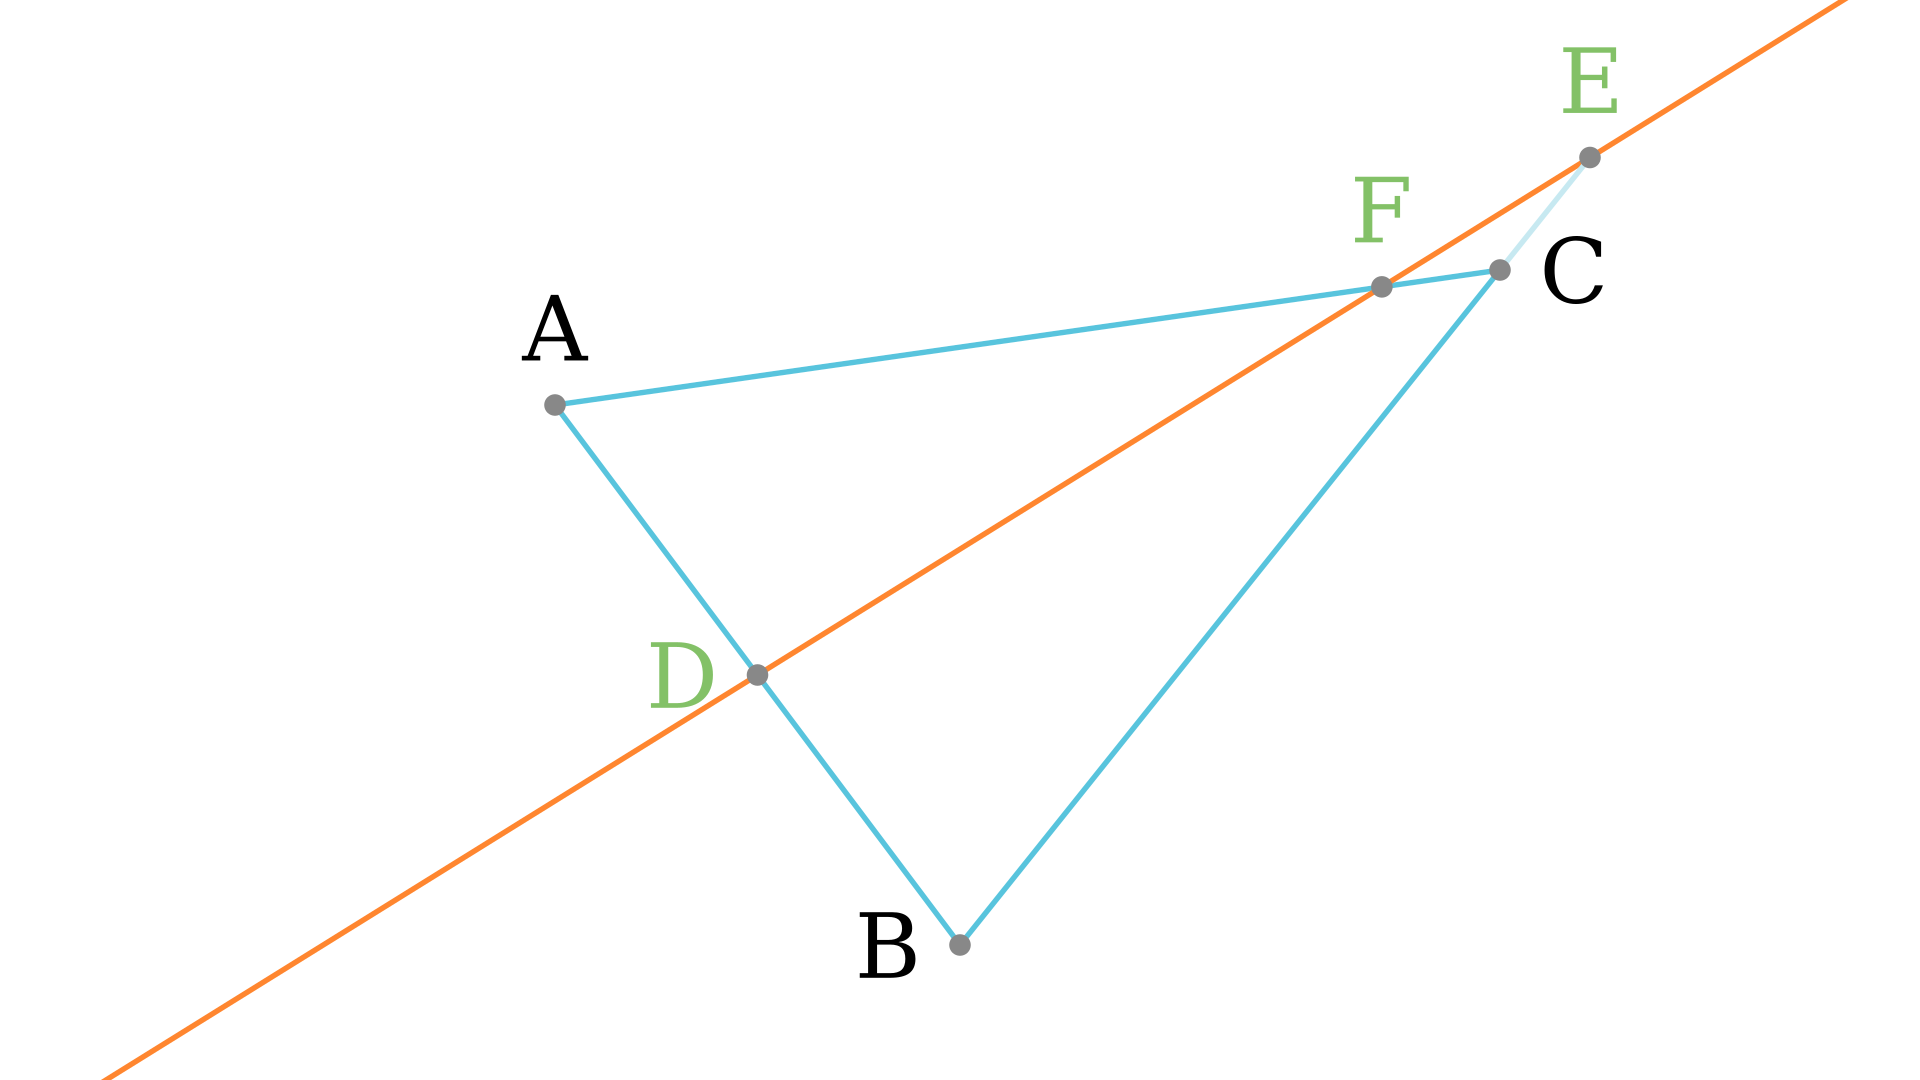
\includegraphics[scale=0.15]{MenelausIllustration.png}
	\caption{Menelaus's theorem}\label{F:menelaus}
\end{figure}

Consider a triangle with vertices \(A\), \(B\) and \(C\) and a line that crosses the (possibly extended) edges \(AB\), \(BC\) and \(CA\) 
of the triangle at points \(D\), \(E\) and \(F\) respectively, as in Figure~\ref{F:menelaus}. Menelaus's theorem states that

$$
	\frac{DA}{DB} \times \frac{EB}{EC} \times \frac{FC}{FA} = 1
$$

This theorem also has a converse, provided certain additional conditions are satisfied -- if \(D\), \(E\) and \(F\) are points on the (possibly extended) edges of the triangle \(ABC\), and either exactly one or exactly three of these points lie on extended edges, and the points satisfy the above equation, then they are collinear.

Note that the additional condition of either exactly one or three of the points being contained on extended edges is automatically satisfied in the first statement.

The above theorem is also valid when signed distances are used in place of regular distances (with signed distances, the line segments \(AB\) and \(BA\) have the same length but differ in sign). In this case, the extra condition is not required for the converse to be true.

\subsection{Formulating Menelaus's theorem using polynomial (in)equations}

Like Pappus' theorem, Menelaus's theorem is solved by formulating it in coordinate geometry, and then as a system of equations and inequations in real variables.

\subsubsection{Defining the variables}

Three distinct points representing the vertices of the triangle \(ABC\) are arbitrarily chosen (one could optimise this by scaling and shifting the triangle to make two of the three vertices coincide with points \((0, 0)\) and \((1, 1)\) on the plane).

A line passing through two points \(P\) and \(Q\) on the plane can be parameterised by a single real number \(l\). Moreover, this parameterisation can be chosen such that the value \(l = 0\) corresponds to the point \(P\) and \(l = 1\) corresponds to the point \(Q\).

The three edges of the triangle -- \(AB\), \(BC\), \(CA\) -- can be parameterised in this manner by real numbers \(r\), \(s\) and \(t\).

Since the theorem requires the transversal line to cross all three edges of the triangle, the points of intersection -- \(D\), \(E\), \(F\) -- correspond to some values of the parameters \(r\), \(s\) and \(t\).

After defining the nine variables (six for the vertices of the triangle and three for the parameters of the edges) required to describe the setup in coordinate geometry, the next step is to formulate a system of equations describing the theorem.

\subsubsection{Equations and inequations}

For the \emph{forward} part of the theorem statement, the hypothesis is that the three points of intersection -- \(D\), \(E\) and \(F\) -- are collinear. As mentioned above, collinearity can be formulated as a polynomial equation in terms of the coordinates of the three points.

The statement of Menelaus's theorem holds even when the regular Euclidean distances (given by $\sqrt{(x_1 - x_2)^2 + (y_1 - y_2)^2}$ for points $(x_1, y_1)$ and $(x_2, y_2)$) are replaced by the squares of the Euclidean distances ($(x_1 - x_2)^2 + (y_1 - y_2)^2$). The equation in the theorem can also be rewritten as

$$
	DA \times EB \times FC = DB \times EC \times FA
$$

With these simplifications, the forward part of the theorem can be expressed as a polynomial in all the variables involved.

The converse (or \emph{reverse}) statement has the additional requirement that the either exactly one or exactly three of the intersection points lie on the extensions of edges of the triangle. Due to the way the parameterisation of the lines was chosen, a point lies on an extended edge if and only if the corresponding value of the parameter is \emph{not} contained in the \(\left[0, 1\right]\) interval.

The condition of a parameter $l$ being contained in the \(\left[0, 1\right]\) interval can be formulated in terms of inequations

$$
	(0 < l) \wedge (l < 1)
$$

The converse of the theorem requires that out of the three parameters \(r\), \(s\), and \(t\), an odd number of them (either one or three) must \emph{not} satisfy the above condition.

This can be captured using the \texttt{XOR} (exclusive \texttt{OR}, which is $true$ when exactly one of the inputs is $true$) function ($\oplus$) --

$$
	\neg \left( \left( (0 < r) \wedge (r < 1) \right) \oplus \left( (0 < s) \wedge (s < 1) \right) \oplus \left( (0 < t) \wedge (t < 1) \right) \right)
$$

which is \(true\) only when an odd number of points lie on the extended edges.

With these modifications, the statement of the theorem can be given to the \texttt{Z3} solver in the form of a system of constraints and polynomial (in)equations over the reals.
The theorem is true if the negation of the theorem statement is unsatisfiable.

\section{Running \texttt{SMT} solvers}\label{running-smt-solvers}

High-performance \texttt{SMT} solvers such as \texttt{Z3} use a huge collection of algorithms, which they
choose and mix using complex heuristics to decide whether a collection
of constraints is satisfiable. When asked to check satisfiability, one of three possible
results is returned -- \texttt{sat}, \texttt{unsat} and \texttt{unknown}, corresponding to
the problem being satisfiable, unsatisfiable and the chosen algorithm failing to answer
the problem. A fourth possibility is manual interruption (i.e., the user giving up) if the solver appears to be failing
to answer -- which is a variant of \texttt{unknown} (indeed if a timeout limit is reached \texttt{unknown} is returned).

In addition, an \texttt{SMT} solver can be asked for a
\emph{proof} in case a problem is not satisfiable (i.e., a proof that
the problem has no solution) or a \emph{model} -- values for variables
that satisfy the constraint -- in case the problem is satisfiable.

\subsection{First attempt: proving Pappus theorem}

When asked to solve the satisfiability problem \emph{with proof},
neither of the \texttt{SMT} solvers \texttt{Z3} and \texttt{CVC4} was able to
prove the Pappus hexagon theorem. This was in spite of our (non-expert)
attempts at changing their parameters to raise various limits,
and allowing them to run for hours.

To try to assess how far they were from proving the theorem, we attempted
a simpler variant. Instead of having all six of \(u\), \(v\), \(x_A\),
\(y_A\), \(U\) and \(V\) as variables (so proving the result for all
values of these), we added additional equations fixing some of them.
Since all but \(x_A\) were known to be positive, for convenience,
conditions could only be added by choosing random positive numbers
corresponding to some of the five variables \(u\), \(v\), \(y_A\), \(U\)
and \(V\) and adding corresponding equations -- for example, we could
pick \(c > 0\) at random and add the equation \(u = c\).

When all \(5\) of the variables were fixed (leaving only \(x_A\) to
vary), \texttt{Z3} solved the problem instantly. When \(4\) of the \(5\) were
fixed, the theorem was proved in about 6 seconds. However, when only
\(3\) were fixed we could not get either solver to prove the result, in
spite of changing parameters.

\subsection{Next attempts: solving (but not proving) Menelaus's theorem}

Our next attempt (using a different program to interface with \texttt{Z3}) was Menelaus's theorem,
formulated as a satisfiability problem contradicting the
statement, as sketched above. When run \texttt{Z3} instantly solved the satisfiability problem
with \texttt{unsat} as the answer (as needed to obtain a contradiction).

But there was a twist to the tale. When we used the same setup as that for the Pappus theorem,
\texttt{Z3} failed to solve the problem (when running for about 10
minutes). Some experimentation revealed the crucial difference between
the two programs was that in the former we were asking for a proof.

Indeed, when the code for Menelaus's theorem was modified to ask for a
proof, \texttt{Z3} ran for a few seconds and returned \texttt{unknown} --
presumably the system was forced to use an algorithm that returned a
proof when the problem was not satisfiable, and this algorithm found the
problem too hard.

\subsection{Pappus revisited}

Based on the above, it was natural to try to ask \texttt{Z3} whether the
constraints corresponding to the Pappus theorem were satisfiable,
without asking for a proof. Another change made, again based on the
above experiments, was to not specify the \emph{logic} to be used.

When run in this way, \texttt{Z3} solved the problem instantly (in 0.02 seconds).



\section{Conclusion: solved but not proved?}

The above experiments showed that when asked for a proof, the choice of algorithms by \texttt{Z3}
was different, either taking much longer (effectively not terminating),
or explicitly giving up.

As we have seen, when asked only for a solution, \texttt{Z3} could quickly and correctly solve the
satisfiability problems corresponding to the two theorems.
Thus, to the extent that \texttt{Z3} can be trusted, we can readily check if
problems of this complexity from Euclidean geometry, and presumably many
other areas, are correct. Even without getting a proof this is valuable
-- at the least avoiding time and effort being spent on what is not
true, and identifying related statements that are true.

The failure to solve with proofs suggests that, at least at present, we cannot hope to
prove non-trivial Euclidean geometry theorems (without trusting \texttt{Z3}) by simply translating
them and using \texttt{SMT} solvers. However, with the underlying solvers rapidly
improving, the solutions in principle may become solutions in practice.
This is especially the case if the algorithms are successfully
parallelized -- to our surprise we observed that the algorithms were
essentially serial even when configured to be parallel, with occasional
use of \(2\) cores being the only concurrency.

It would also be interesting to see in greater detail what causes such
algorithms to be so slow, say with the above model problems. In
particular, while it is known that in the worst case any algorithm must
be slow, perhaps there are special features in cases of interest that
allow speeding up.

\section*{Appendix: running \texttt{Z3} and the \texttt{SMT} format}

\begin{figure}
	\begin{lstlisting}[language=LISP, frame=single]
(declare-fun u() Real)
(declare-fun v() Real)
(declare-fun Ax() Real)
(declare-fun Ay() Real)
(declare-fun U() Real)
(declare-fun V() Real)
(declare-fun Px() Real)
(declare-fun Py() Real)
(declare-fun Qx() Real)
(declare-fun Qy() Real)
(declare-fun Rx() Real)
(declare-fun Ry() Real)
(assert (= (* (- Py 0.0) (- (* Ax (+ U 1.0)) 1.0)) 
	(* (- (* Ay (+ U 1.0)) 0.0) (- Px 1.0))))
(assert (= (* (- Py Ay) (- (+ 1.0 u) Ax)) 
	(* (- 0.0 Ay) (- Px Ax))))
(assert (= (* (- Qy 0.0) (- (* Ax (+ (+ U V) 1.0)) 1.0)) 
	(* (- (* Ay (+ (+ U V) 1.0)) 0.0) (- Qx 1.0))))
(assert (= (* (- Qy Ay) (- (+ (+ 1.0 u) v) Ax)) 
	(* (- 0.0 Ay) (- Qx Ax))))
(assert (= (* (- Ry 0.0) (- (* Ax (+ (+ U V) 1.0)) 
	(+ 1.0 u))) (* (- (* Ay (+ (+ U V) 1.0)) 0.0) 
	(- Rx (+ 1.0 u)))))
(assert (= (* (- Ry (* Ay (+ U 1.0))) (- (+ (+ 1.0 u) v) 
	(* Ax (+ U 1.0)))) (* (- 0.0 (* Ay (+ U 1.0))) 
	(- Rx (* Ax (+ U 1.0))))))
(assert (> u 0.0))
(assert (> v 0.0))
(assert (> Ay 0.0))
(assert (> U 0.0))
(assert (> V 0.0))
(assert (not (= (* (- Qy Py) (- Rx Px)) 
	(* (- Ry Py) (- Qx Px)))))
(check-sat)
\end{lstlisting}
	\caption{SMT format for Pappus theorem}\label{smt-pappus}
\end{figure}

\texttt{SMT} solvers such as \texttt{Z3} can be run from many languages (in case of \texttt{Z3} we
can use Python, C++, Java and other JVM languages such as Scala). But
one nice way to run these, and especially to examine the problems being
solved, is to use a standard format called \textbf{\texttt{SMT2}} which all \texttt{SMT}
solvers support (this can be run interactively or as a file from the
command line).

As an example, we give the \texttt{SMT2} code for the Pappus problem in Figure~\ref{smt-pappus}. This is a language
with syntax (following LISP/Scheme) that is easy for both machines and
people to read. Each statement is a so called \textbf{S-expression}
(i.e., symbolic expression), which is a list enclosed in parenthesis.
Operators and functions come in the beginning, so we write, for example,
\texttt{(+\ 2\ 3)} for \(2 + 3\) and \texttt{(=\ (+\ 2\ 3)\ (+\ 3\ 2))}
for \(2 + 3 = 3 + 2\). In general, an S-expression is a list, enclosed
in parenthesis with entries either other S-expression or \textbf{atoms},
with atoms being integers, reals, strings, functions, operators etc.

Specifically, most of our statements are of one of two forms --
declaring a variable using \texttt{declare-fun} (which can more
generally be used to declare functions), or asserting conditions using a
statement \texttt{(assert\ <expression>)} for a
Boolean expression.

	{\small
		\begin{figure}
			\begin{lstlisting}[language=Python, frame=single]
def are_collinear(p, q, r):
  return ((q[1]-p[1])*(r[0]-p[0])==(r[1]-p[1])*(q[0]-p[0]))

def d(p, q):
        return (p[0]-q[0])**2 + (p[1]-q[1])**2

menelaus_theorem = Implies(And(Not(are_collinear(A, B, C)), 
  are_collinear(D, E, F)), 
  d(A, D) * d(B, E) * d(C, F) == d(D, B) * d(E, C) * d(F, A))
\end{lstlisting}
			\caption{Extract of Python code for Menelaus's theorem}\label{python-menelaus}
		\end{figure}
	}

Incidentally, we have run \texttt{Z3} in a few ways -- using Python, using Scala
via the Java API and using Scala to generate code in the \texttt{SMT2} language
(like the above code) and using the \texttt{Z3} command line either
programmatically or in a terminal. The interfaces in high-level
languages are also pleasant and human readable. For instance, an extract
from the Python code for Menelaus theorem is in figure~\ref{python-menelaus}



\begin{thebibliography}{10}

	\bibitem{Ar} Artin, Emil
	\textit{Geometric Algebra},
	Dover.

\end{thebibliography} \end{document}

